\section{Q2} 

\subsection{Introduction} \label{sec:Introduction}

In the context of industrial automation, conveyor belt systems play a crucial role in material handling processes, 
ensuring continuous and efficient movement of goods within a production line. The objective of this laboratory task 
is to design, simulate, and analyze an electromagnetic control system to manage the operation of a conveyor belt, 
driven by a single-phase AC induction motor.

The system's functional specifications demand a controlled startup delay, immediate stoppage via a stop push 
button, and an automatic halt upon the activation of a limit switch sensor. To meet these requirements, the 
control architecture integrates key components such as a general magnetic circuit breaker, a thermal relay, 
a lamp emulator, and push buttons configured with normally open (NO) and normally closed (NC) contacts.

This report outlines the design process, starting with the development of a Grafcet diagram representing the 
sequence of operations, followed by the assembly diagram detailing the connections between components. From this, 
both the electrical power and command circuits are derived. Finally, the proposed system is simulated using 
Fluidsim 3.6 to verify that it meets the operational specifications. Through this exercise, essential concepts 
of electromagnetic technology applied to industrial control systems are reinforced, with emphasis on safety, 
responsiveness, and process reliability.

\subsection{Grafcet Representation} \label{sec:Grafcet_Representation}

\begin{figure}[H]
    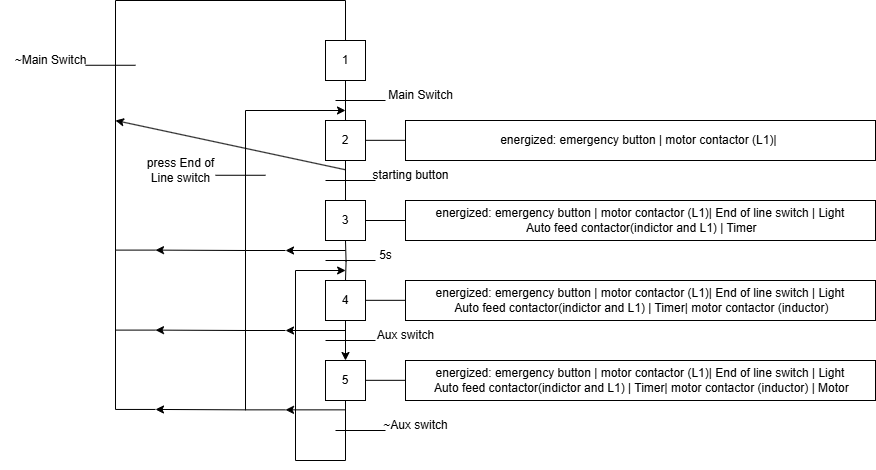
\includegraphics[width=16cm]{Images/Q2/grafset.png}
    \centering
    \caption{Grafset for industrial plant motor}
    \label{fig:grafset_complex}
\end{figure}

\subsection{Process Schematic and Sensor-Actuator Integration} \label{sec:Process_Schematic_and_Sensor-Actuator_Integration}

\begin{figure}[H]
    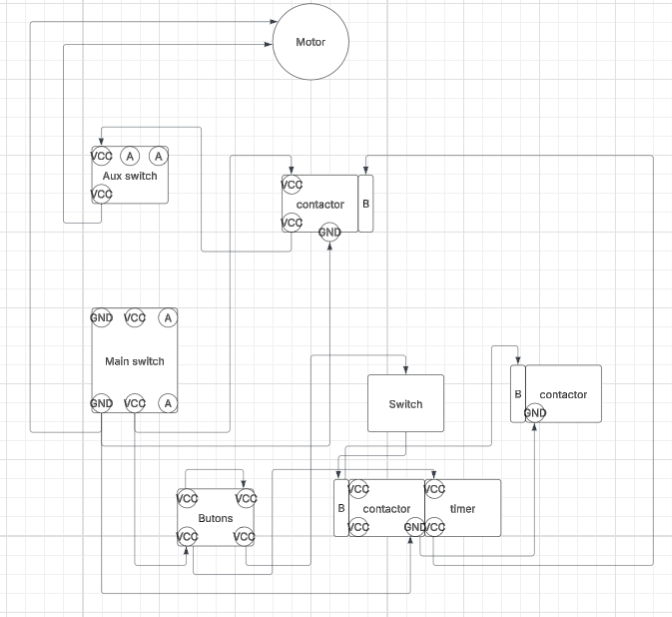
\includegraphics[width=16cm]{Images/Q2/eletrical_circuit.png}
    \centering
    \caption{Eletrical circuit of industrial plant motor}
    \label{fig:eletrical_circuit}
\end{figure}

\subsection{Electrical Power Circuit Diagram} \label{sec:Electrical_Power_Circuit_Diagram}

\begin{figure}[H]
    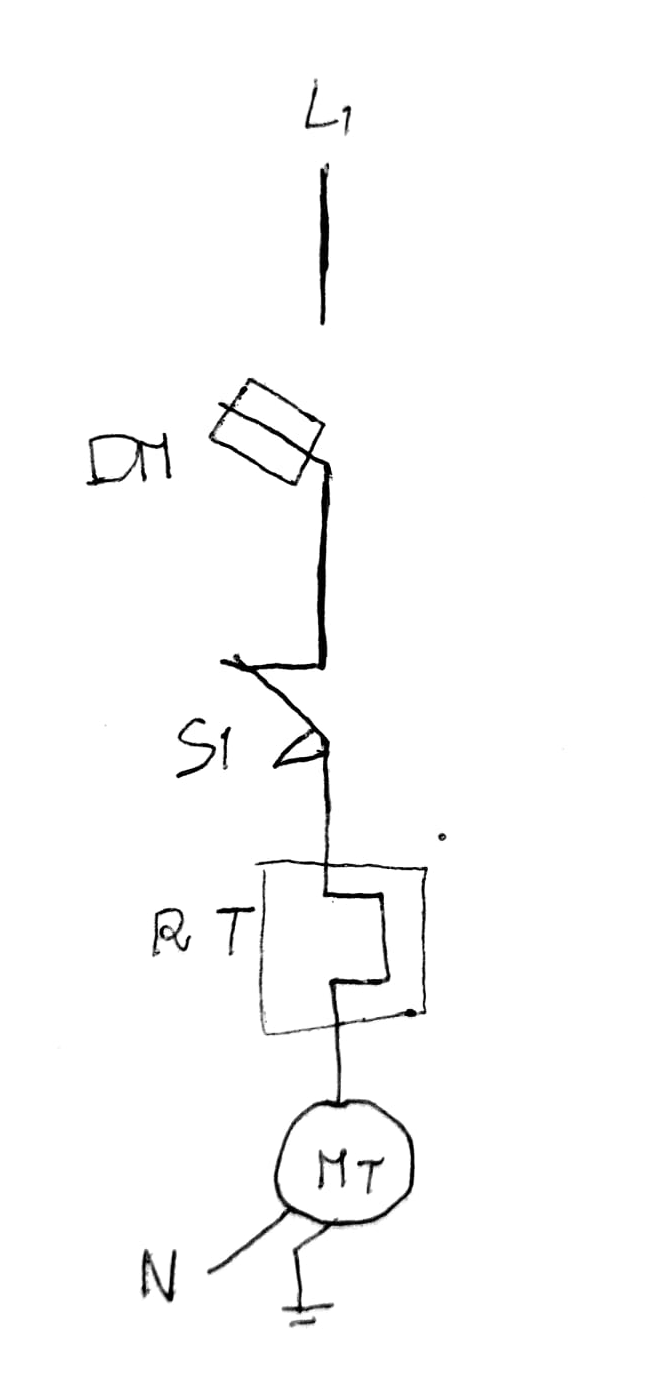
\includegraphics[width=16cm]{Images/Q2/Q2_power.jpeg}
    \centering
    \caption{Power Circuit for Q2 system}
    \label{fig:Q2_power}
\end{figure}

\subsection{Electrical Command Circuit Diagram} \label{sec:Electrical_Command_Circuit_Diagram}

\begin{figure}[H]
    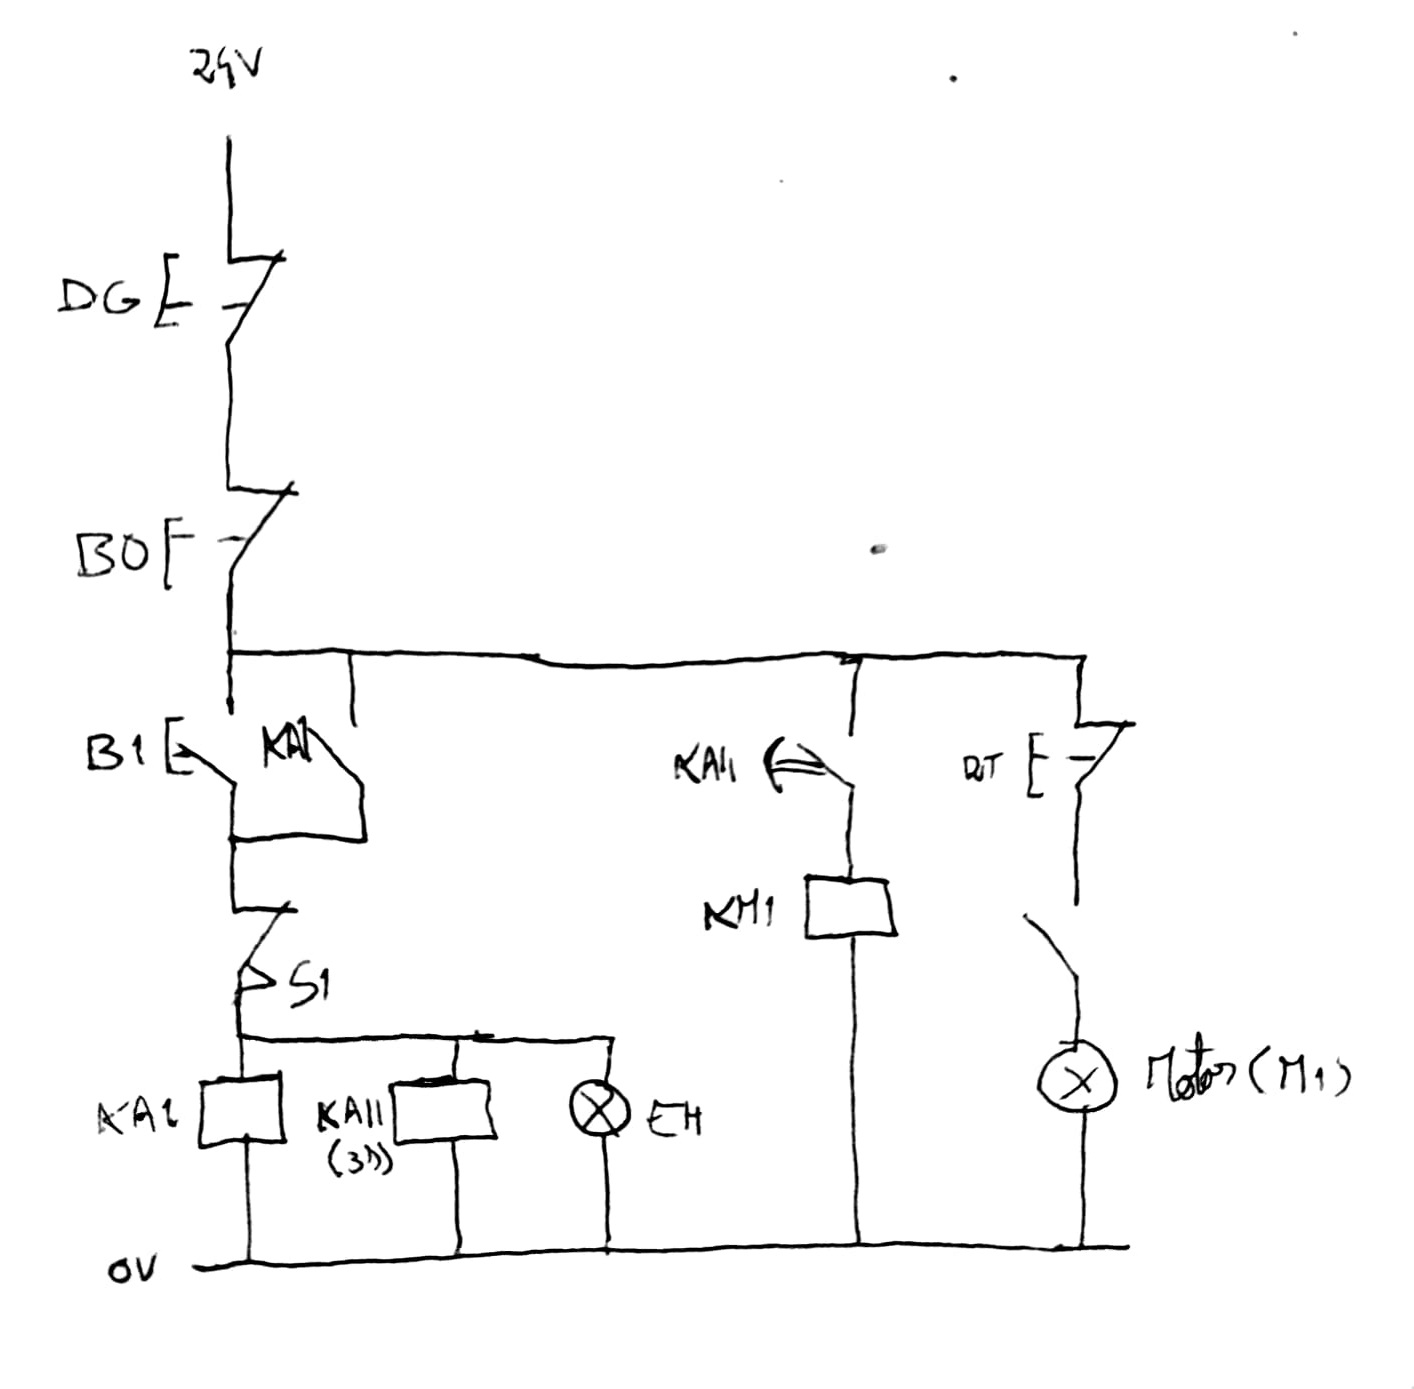
\includegraphics[width=16cm]{Images/Q2/Q2_command.jpeg}
    \centering
    \caption{Command Circuit for Q2 system}
    \label{fig:Q2_command}
\end{figure}

\subsection{Simulation and Validation} \label{sec:Simulation_and_Validation}

\begin{figure}[H]
    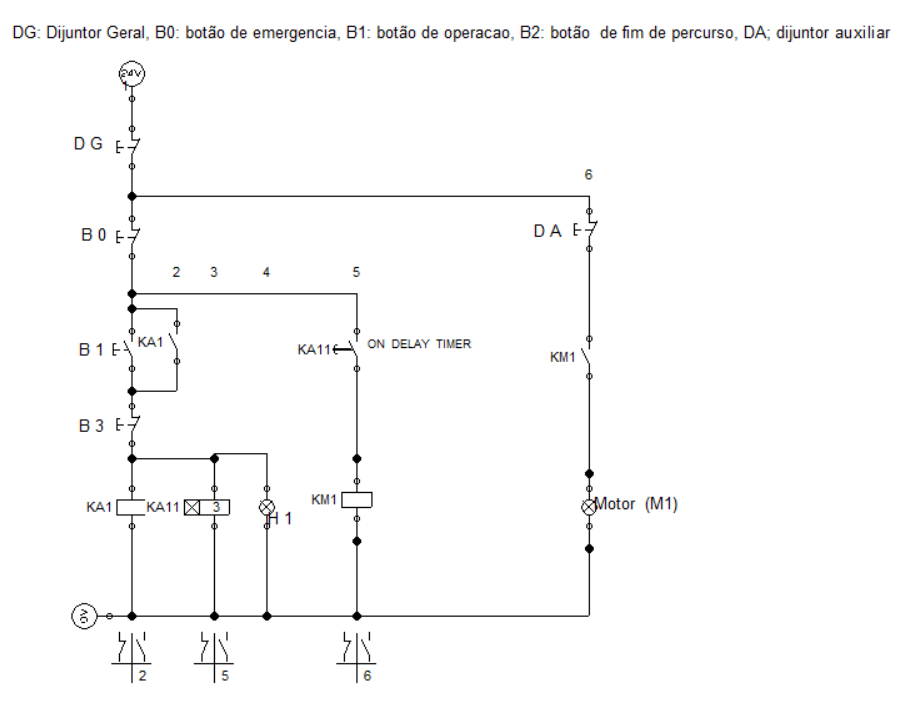
\includegraphics[width=16cm]{Images/Q2/fluidsim.png}
    \centering
    \caption{Fluidsim for the motor control}
    \label{fig:fluidsim}
\end{figure}

\subsection{Conclusion}

This report details the complete development of an electropneumatic control system, from schematic 
design to simulation validation. By integrating various automation components and methodologies, 
the system achieves a robust and efficient control mechanism. The findings highlight the importance 
of precise component selection and control logic design in achieving a functional and reliable 
automated process.